\subsection{Performance}

This section will explore the performance characteristics shown by all of the SUTs and will answer the research questions proposed in \autoref{section:req-cap-performance}. Furthermore, the optimisations introduced in \autoref{section:optimisations} will be explored to determine which configurations are optimal and when.

This investigation will be conducted in two steps. First, the generalised performance across all tests will be explored for each emulator; this can be done by observing the relationship between different test statistics (such as performance vs hotness). From this the ideal configuration for each emulator will be determined.

Next, the performance will be investigated more thoroughly on the bespoke set of test suites. Unlike the functionality tests, these test suites are specifically designed to stress the SUTs in different ways and have been designed to answer the various performance research questions. The test suites of interest are as follows:

\begin{itemize}
    \item \textbf{\texttt{fibonacci(n)}}
    
    Recursive program that computes \texttt{fibonacci(n)} designed to explore the performance of highly recursive program. Uses a mixture of ALU and memory operations. The computational complexity is $\mathcal{O}(2^n)$ and thus we can expect to see very long and intensive tests for larger $n$.
    
    \item \textbf{\texttt{fibonacci\_rep[10](n)}}
    
    The same as \texttt{fibonacci(n)}, however 10 unique instantions of the \texttt{fibonacci} function are generated. This helps investigate how performance scales with more unique code.
    
    \item \textbf{\texttt{fibonacci\_rep[100](n)}}
    
    The same as \texttt{fibonacci\_rep[10](n)} but with 100 unique instantions.
    
    \item \textbf{\texttt{factorial(n)}}
    
    Recursive program that computes \texttt{factorial(n)}. Since the complexity is $\mathcal{O}(n)$ and $n!$ grows exponentially with respect to $n$, this test suite will not lead to long intensive tests.

    \item \textbf{\texttt{memcpy(n)}}
    
    Iterative program that copies $n$ bytes from one location in memory to another. The very high proportion of memory instructions touching a large space of memory will stress the memory map.
    
    \item \textbf{\texttt{memcpyw(n)}}
    
    The same as \texttt{memcpy(n)} however words will be touched and copied instead of individual bytes.
    
    \item \textbf{\texttt{primal(n)}}
    
    An iterative program that determines if $n$ is primal. With no memory instructions present this should result in a very hot ALU heavy loop. Since the complexity is $\mathcal{O}(n)$, the values of $n$ supplied to the test suite will grow on the order of $2^n$; all values of $n$ used will be primal.
    
    \item \textbf{\texttt{unroll(n/m)}}
    
    A program loop of $n$ iterations that has been unrolled into $n/m$ chunks such that the unrolled program has $m$ iterations. Designed to investigate how the trade-off of unrolling varies with each SUT.
\end{itemize}

\YIComment{Redo this}

\YIComment{Include hybrid in comparisons}

\YIComment{Talk about fib\_rep tests}

\YIComment{Talk about compilation inefficiency graph}

\YIComment{Move hotness stuff into subsubsection}

\autoref{figure:time-jit-interpreter} shows that the interpreter has far better performance than the JIT for short tests. As the test duration increases the JIT increases in performance, eventually stabilizing at approximately 2x faster execution time than the interpreter.

\autoref{figure:hotness} illustrates the relationship between program hotness and emulation performance. It shows that for the JIT emulator, performance rapidly increases as the hotness does. This is because each block has a fixed compilation cost, which is further amortized the hotter it is, resulting in higher performance. The interpreter on the other hand is unable to see the same improvement as the associated costs for a given block are required for every execution and cannot be amortized.

\begin{figure}[H]
    \centering
    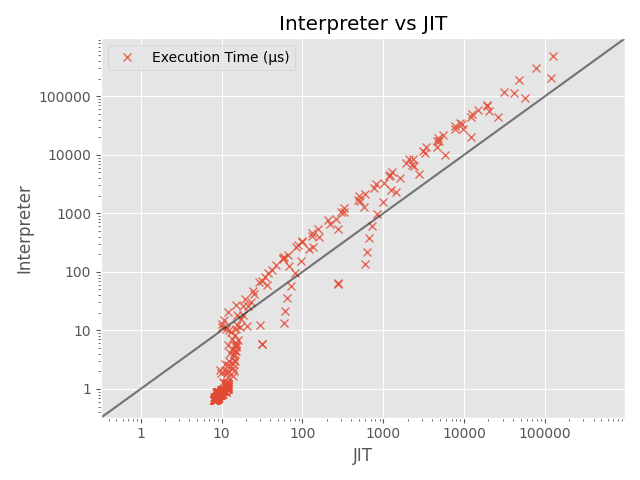
\includegraphics[scale=0.75]{output/graphs/scatter/vs/JIT-vs-Interpreter-time.png}
    \caption{Execution time of all tests for the JIT against the interpreter.}
    \label{figure:time-jit-interpreter}
\end{figure}

\begin{figure}[H]
    \centering
    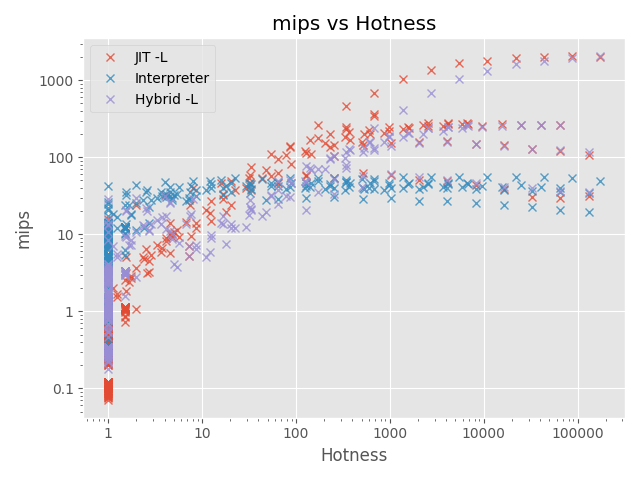
\includegraphics[scale=0.75]{output/graphs/scatter/emulators/hotness.png}
    \caption{Performance against hotness for all tests.}
    \label{figure:hotness}
\end{figure}

\subfile{interpreter}
\subfile{jit}
\subfile{hybrid}
\subfile{iteration}
\subfile{recursion}
\subfile{memory}
